\documentclass{article}
\usepackage[greek,english]{babel}
\usepackage{mflogo}
\usepackage{graphicx}
\languageattribute{greek}{polutoniko}
\newcommand*\ctan{\textsc{ctan}}
\author{Claudio Beccari}
\title{The CB Greek fonts}
\date{1 January 2008}
\usepackage[T1]{fontenc}
\usepackage{lmodern}
\DeclareFixedFont{\Did}{LGR}{cmr}{m}{n}{10}
\newcommand*\uishape{\fontshape{ui}\selectfont}
\newcommand*\lishape{\fontshape{li}\selectfont}
\newcommand*\rsshape{\fontshape{rs}\selectfont}
\newcommand*\roshape{\fontshape{ro}\selectfont}
\newcommand*\ivshape{\fontshape{iv}\selectfont}
\newcommand*\uvshape{\fontshape{uv}\selectfont}
\newcommand*\cbtext{abgdezhjiklmnxoprstufqyws}
\newcommand*\cbtest[1][]{\foreignlanguage{greek}{#1\cbtext}}
\begin{document}
\maketitle
\begin{abstract}
This is the documentation accompanying a revision of the CB Greek fonts completed on the 1st January 2008. It comprises the instructions for installing the fonts and describes their various features. 
\end{abstract}

\section{Introduction}
The CB Greek fonts have been in free use by the \TeX\ community for years now; the bitmapped fonts were available by the end of the '90s, while the scalable Type~1 versions started to be available in 2002; some new fonts were added in the following years, but in 2005 a fundamental change was made: the Type~1 versions were reduced to the only size of 10\,pt, redone completely and associated to a correct encoding vector by Apostolos Syropoulos, who, in a sense, is a co-author of this collection of fonts. I wrote the \MF\ code; he and many other Greek users assisted me in the correction of errors or in a better rendering of specific glyphs.

The whole work had started from the Greek fonts designed by Silvio Levy several years before; they are still available and can be found in the \ctan\ archives and are being maintained.

When I started working on this project I wanted to create a full set of fonts that could match completely the EC Latin fonts; the latter had been available in the second half of the '90s, although only in bit map form. The need for Type~1 version did exist, but the tools to convert \MF\ fonts into Type~1 ones were still rudimentary, in spite of the hard work that many people had spent in creating them. In any case the collection of the CB fonts contained the three families (roman, sanserif, typewriter), two series (medium and bold extended) and four shapes (upright, slanted, italics, small caps) that were standard with \LaTeX\ at that time. During the creation of the font some requests were set forth, so that an outline family was added, the original ``italic'' shape was enriched with an alternative derived from the types used by the Teubner Typesetting Company of Lipsia; the slanted shape of the two italics was completed with the upright italics, and the small caps were duly completed with the bold versions. Of course also the corresponding fonts for the \texttt{slides} class were prepared. Eventually, for typesetting classical Greek philology works, another font was created, mainly for typesetting the metric schematic characteristics of ancient Greek poetry.

The standard sizes for the text EC fonts were 5, 6, 7, 8, 9, 10, 10.95, 12, 14.4, 17.28, 20.74, 24.88, 29.86 and 35.83 points; while the standard sized for the slides fonts were 7, 8, 10, 12, 13.82, 16.59, 19.91, 23.89, 28.66, 34.4, 41.28 points. Combining all these sizes with the family, series and shape of the various fonts approximately 900 driver files were prepared and this distribution contains the corresponding \TeX\ metric files and the Type~1 renderings for a total of approximately 2800 files.

When in 2005 the Type~1 fonts were reduced to the 10\,pt size only, the \ctan\ decided to keep the old version of the complete collection; for one reason or another, this statement remained true only for the \MF\ related material, but not for the Type~1 fonts.

This redistribution of the full collection of fonts was redone completely from the original \MF\ sources, with no modifications or corrections whatsoever, but  the \TeX\ metric files were redone with the latest distribution of \MF, and the Type~1 fonts were completely redone with modern means, and the encoding vector created by Apostolos Syropoulos was used as the internal encoding of these fonts.

The initial version of the pfb files were obtained very laboriously by Apostolos by means of \textsf{TeX-trace}, the best tool that could be used at the beginning of this decade. Some of the fonts, added in a second time in 2004, were done with a new tool, \textsf{mftrace} by Han-Wen Nienhuys. Years ago also \textsf{mftrace} (at that time called \textsf{pktrace}) resorted to the same tracing algorithm used by \textsf{TeX-trace}, so that the results were absolutely comparable, but the amount of manual work was definitely smaller; nowadays \textsf{mftrace} resorts to a new tracing program, \textsf{potrace} by Peter Selinger; this new algorithm appears to be faster and to produce better outlines, at least to the point that the corresponding pfb files are some 10\% smaller than those obtained with \textsf{TeX-trace}. With the previous algorithm and with the actual one, \textsf{mftrace} can resort to the program \textsf{FontForge} by George Williams; this latter program can be used as a filter and can perform some postprocessing on the obtained fonts without triggering the GUI, but working in the background.

The result is that with a proper script for generating the whole set of about 900 transformations from the \MF\ source to the final pfb files, the total amount of time I spent on my laptop was some 5h45min of unattended processing, while I was enjoying the 2007 New Year's Eve with my family and friends.

\section{Installation}
I suggest you to install everything concerned with the CB Greek fonts into your local tree, unless your \TeX\ system comes with the fonts already installed. Evidently in this case you don't need to perform any installation. Nevertheless I suppose that the standard \TeX\ system distributions by default come only with the 10\,pt size; therefore if you put this complete installation into your personal or local tree, this becomes dominant with respect to the system tree and you need not worry about the distribution.

\subsection{Discovering if the full installation is already installed}
In order to see if the full complete installation is alreeady on your system you can act in different ways, but I suggest you to do the following.

Create yourself a small file such as this one:
\begin{verbatim}
% file test-cbgreek.tex
\documentclass[12pt]{article}
\usepackage[greek]{babel}
\usepackage[T1]{fontenc}
\begin{document}
Qa'ire!
\end{document}
\end{verbatim}
and run it through \textsf{pdflatex}; after the run, either in the suitable window of your GUI, or by opening the test-cbgreek.log file, examine if the 12\,pt font was chosen from the installed full collection or if, lacking this font, a bitmapped version has been created on the fly during the \textsf{pdflatex} run. In the latter case you are sure you installation is not the full one.

Now try again by modifying and changing name to the above little file as such:
\begin{verbatim}
% file test-cbgreek10pt.tex    <----- !
\documentclass[12pt]{article}
\usepackage[greek]{babel}
\usepackage[T1]{fontenc}
\usepackage[10pt]{type1ec}%    <----- add this line
\begin{document}
Qa'ire!
\end{document}
\end{verbatim}
If this time the final list of fonts embedded in the final pdf document lists the use of the font grmn1000.pfb, then your installation contains the reduced set of 10\,pt fonts and scales them to the typesetter's needs, to 12\,pt in our example. If  the font list at the end of the log file still makes reference to the pk fonts with a font name such as grmn1200.600pk, then your installation contains the \MF\ machinery, but the Type~1 fonts are not installed or there is something missing in their configuration. If with either experiment you find out that your \TeX\ system installation does not contain the full CB Greek font collection, you need to install it.

Nevertheless with the second experiment you know what you have to do in order to use only the reduced 10\,pt set; may be the kind of documents you write does not require a full installation; in case, the following subsection tells you what to do.

By the way, the compiled pdf document should contain only the word \foreignlanguage{greek}{Qa'ire!} that, of course, means ``Hallo!''

\subsection{Installing the full collection}
\subsubsection{Copy the folders}
After decompressing the archive, action that I assume already done, otherwise you'd not be reading this document, copy the whole fonts folder to your local tree and the whole tex folder to your local tree. Copying means that you might need to point and drag the above folders in the root of your local tree; if the folders already exist your operating system should be smart enough not to make duplicates, but to ask you if you want to put the contents of the dragged folders into the already existing ones; possibly your operating system will ask you again such question, in case the sub folders already existed; possibly, if you repeat the whole operation without recalling that you already did it, the operating system should inform you that files with the same name already exist in the specified folders and if you want to replace them with the new ones.

\subsubsection{Refresh the file name database}
As a second step you should refresh the file name data base; this operation is done differently in the various \TeX\ system distributions:
\begin{itemize}
\item With MiK\TeX\ on Windows platforms you have to click on Start, then MiKTeX, and then MiKTeX Options, and select the button labelled Refresh File Name Database.
\item On Linux and similar systems open the console and change directory to the root of your local/personal tree, very likely in \verb|~/texmf|. Then execute the command \verb|texhash ./|
\item On Mac OS X you don't need to do anything because your personal tree is rooted in your \verb|Library/texmf| folder, and everything in the \verb|Library| folder and its sub folders is automatically on the search path of every Mac application, at least of the \TeX\ system.
\end{itemize}

\subsubsection{Create the maps}
The next step is required for using the Type~1 fonts and is very delicate; the details vary from one \TeX\ system distribution to another, but if you are willing to use the command line interface it should not be so difficult to do.

\begin{enumerate}
\item Copy the \verb|updmap.cfg| file from the system tree branch \texttt{web2c} to a folder with the same name grafted the same position in your local/personal tree;
\item edit the copied file so as to change the \texttt{cbgreek.map} name to \texttt{cbgreek-full.map}; control that the line you modified does not contain any comment mark, that in that file is made up by the hash sign \texttt{\#}; the word \texttt{Map} or \texttt{Mixedmap} should be flush left;   save the modified file;
\item from the same location run the program\footnote{With some systems you should prefix the command \texttt{updmap} with its full path, in case its folder is not on the search path for the operating system; on some systems \texttt{./} is redundant or must be changed into \texttt{.\char92}; if you know what operating system you are using and you know how to display the system path, you should not have any difficulty in adapting the following command to your particular situation.}
\begin{flushleft} 
\verb+updmap --cnffile ./updmap.cfg+
\end{flushleft}
\item While \verb|updmap| is doing its work, it will typeset everything it's doing on the screen and will finish informing you that a certain number of map files have been created.
\item Check the outcome of the above procedure by opening the newly created \texttt{pdftex.map} and search if it contains, say, the reference to the font \texttt{grmn1200.pfb};
\item if it does, another run on the source file \texttt{test-cbgreek.tex} will confirm you that you have available the cbgreek fonts in all sizes and that you can correctly use them. If it does not, there is something wrong with your \TeX\ system distribution: may be an obsolete one? No problem; read the documentation that comes with it and do accordingly; probably you have simply to move the files around in other folders or your executable programs have different names.
\end{enumerate}

\section{Customizations}
The font description files included in the local \texttt{tex/latex/cbgreek} folder allow to a certain number of customizations; may be in the future it will be available a \LaTeX\ extension file, say, \texttt{cbgreek.sty} to call with its options from the main \LaTeX\ source file of your document, so as to select which ``roman'' Greek font you want; you have the choice 
\begin{enumerate}
\item between the traditional Didot Design \cbtest\ and the Greek fonts with ``roman'' serifs \cbtest[\rsshape];
\item between the imitation of the Olga italics \cbtest[\itshape] or the Lipsian ``italics'' \cbtest[\lishape];
\item between the standard sans serif \cbtest[\sffamily\itshape] and the variant \cbtest[\sffamily\ivshape].
\end{enumerate}

In order to chose the fonts you want to use, you should do the following:
\begin{enumerate}
\item if you like the serifed  design more than the Didot design, select the \texttt{rs} shape for upright characters, and the \texttt{ro} shape for the oblique ones.
%
\item If you prefer the more compact Lipsian font to the Olga one, select the \texttt{li} shape; if you are going to use the TX fonts and/or the PX fonts together with the CB ones, you might prefer to use the bold series (b) instead of the  bold extended one (bx) so that with fonts different from the EC ones the simple bold might be preferable; in this case select the \texttt{b} series.
%
\item If you prefer the `arched' epsilon \foreignlanguage{greek}{\sffamily\ivshape e} with sanserif italic fonts instead of the `curly' one \foreignlanguage{greek}{\sffamily\itshape e}, select the \texttt{iv} shape or the \texttt{uv} shape for the oblique or upright sanserif italics respectively.
%
\end{enumerate}

I did not define any command for using the new shapes, but you would not have any difficulty to add in your preamble the two lines:
\begin{verbatim}
\newcommand*{\uishape}{\fontshape{ui}\selectfont}
\DeclareTextFontCommand{\textui}{\uishape}
\end{verbatim}
so as to be able to use the declaration \verb|\uishape| or the text command \verb|\textui| the same as you would use the declaration \verb|\itshape| or the text command \verb|\textit|. You can do the same for selecting the other new shapes concerning the serifed fonts, or the Lipsian italics, or the sanserif variants mentioned above.

But I prepared also the font definition files for using the CB Greek fonts together with the Latin Modern ones. The new shapes are defined in those files; the new commands you defined for your benefit work also when the LM fonts are used for the Latin script. In facts the selection of the Greek alphabet takes place just by changing the font encoding, not the other font characteristics; nevertheless use always high level commands for changing fonts, and never use the real low level family names because the CM/EC family names are different from those pertaining to the LM fonts. In other words do not use \verb|\fontfamily{cmr}\selectfont| for selecting the roman fonts, but use \verb|\rmfamily|, and do the same for the other families. For selecting the outline family use \verb|\outlfamily|.

Pay attention to the fact that the LM fonts use some families, series and shapes that are missing from the EC collection, so that if your default series and shape is missing from the CB fonts, sometimes it gets substituted with something else, and sometimes it gets substituted with the default font, which might even be the usual roman medium upright font; you get messages in the log file, though. At the same time the LM fonts do not contain certain series and shapes that are present in the CB fonts; therefore the available Greek fonts are used, instead of substituting them as it is done with the Latin ones.

\section{Special Greek symbols}
The CB Greek fonts are completed with several different symbols; some of them are used for the Greek numerals; if you want to use the Acrophonic Attic numerals you have to use the \texttt{athnum.sty} package. Otherwise the \texttt{greek} option to the \textsf{babel} package contains all the commands for generating the required symbols; the package contains also a couple of macros for rendering the common decimal integer numbers into the corresponding Greek numerals written with the common alphabet enriched with the symbols `stigma', `qoppa' and `sampi'; the Greek date can be obtained with the specific command \verb|\Grtoday|, and today's date is \foreignlanguage{greek}{\Grtoday}, while the usual modern date is typeset as \foreignlanguage{greek}{\dategreek\today}.

If you are using some implementation of the Latin keyboard, remember that the Greek letters are obtained by striking the similar Latin keys; `similar' is either by sound or by shape; just a couple of letters have a Latin counterpart chosen among the available free Latin keys; refer yourself to table~\ref{tab:transcod} for your convenience.

\begin{table}\let\D\Did\tabcolsep 4.25pt
\makebox[\textwidth]{%
\begin{tabular}{*{25}c}\hline
\D a & \D b & \D g & \D d & \D e & \D z & \D h & \D j & \D i & \D k & \D l & \D m & \D n & \D x & \D o & \D p & \D r & \D s & \D sv & \D t & \D u & \D f & \D q & \D y & \D w \\
a & b & g & d & e & z & h & j & i & k & l & m & n & x & o & p & r & s & s & t & u & f & q & y & w \\\hline
\end{tabular}}
\caption{Correspondence between the Latin keys and the Greek letters}\label{tab:transcod} 
\end{table}

Notice, though, that the final sigma {\Did s} comes out by itself, thanks to the font ligature and kerning table; this means that when the latin `s' is followed by anything different from a letter, which means that the word is finished, the font automatically turns the {\Did sv} into a {\Did s}. This mechanism is so `sticky' that it becomes difficult to type ans isolated {\Did sv}; in order to do so it is necessary to hide the end of the word to the ligature mechanism, and this is done thanks to a letter-strut; in other words the Latin key `v' inserts an invisible strut, the height of a lower case letter without ascenders, but with the category code of a letter. So if you type `\texttt{sv}', the Latin letter `s' is followed by another letter, that does not show on paper or on screen, therefore the `s' is not at the end of a word. At the same time if you are used to type `c' for inputting the final sigma, you can continue to do so: \texttt{l'ogoc} and \texttt{l'ogos} both produce \foreignlanguage{greek}{l'ogos}.

For what concerns the numerous diacritical signs used in Greek, remember that if you do not specify the attribute `polutoniko' to the Greek language, you intend to typeset your input  with the `monotoniko' spelling, and is up to you to avoid rough and smooth spirits (breadths), graves, and circumflexes, but you should stick to the acute accent and the diaeresis. If you want to write polutoniko, you have to specify it with
\begin{verbatim}
\usepackage[...,greek,...]{babel}
\languageattribute{greek}{polutoniko}
\end{verbatim}
With this specification all the signs listed in table~\ref{tab:diacr} can be used for inputting the diacritical signs, even the \verb|~|, that, therefore, can't be used any more as a tie command as in ordinary \LaTeX. The diacritical signs are input in any order, except the subscribed iota, but always before the letter they accompany; \verb+~>a|+ and \verb+>~a|+ both yield \foreignlanguage{greek}{~>a|}; \verb|<roma'ios| yields \foreignlanguage{greek}{<roma'ios}.

\begin{table}[ht]\def\D#1 {\foreignlanguage{greek}{#1}}
\let\t\ttfamily
\centering
\begin{tabular}{*7c}\hline
\D > & \D < & \D "v & \D ~v      & \D ' & \D ` & \D | \\ 
\t > & \t < & \t " & \t \char126 & \t ' & \t ` & \t | \\\hline
\end{tabular}
\caption{Diacritical signs and Latin keystrokes}\label{tab:diacr}
\end{table}


It's necessary to pay attention to the diaeresis sign; it behaves as a diaeresis only if it is followed by a letter; it behaves as an apostrophe if it is after the end of a word; the normal apostrophe key is already used for the acute accent. At the same time when spelling monotoniko you have to type in \verb|a"'ulos| for typing \foreignlanguage{greek}{a"'ulos}, but you can type in \verb|>a'ulos| in polutoniko to get \foreignlanguage{greek}{>a'ulos} (although modern Greeks, even when spelling polutoniko, often use a redundant diaeresis: \verb|>a"'ulos| and get \foreignlanguage{greek}{>a"'ulos} in order to emphasize the hiatus).

Punctuation marks are the usual ones even if they might appear differently; see table~\ref{tab:punct}. Please notice the apostrophe can be obtained both with the double straight quotes and with two single apostrophe signs; the Greek quotation marks, similar to the French `guillemets', are obtained with a ligature of two similar parentheses.

\begin{table}[htb]\let\D\Did\let\t\ttfamily
\centering
\begin{tabular}{*{14}c}\hline
\D , & \D . & \D ; & \D : & \D ! & \D ? & \D -- & \D --- & \D " & \D '' & \D ( & \D ) & \D (( & \D )) \\
\t , & \t . & \t ; & \t : & \t ! & \t ? & \t -{}- & \t -{}-{}- & \t " & \t '' & \t ( & \t ) & \t (( & \t )) \\\hline
\end{tabular}
\caption{Punctuation signs and Latin keystrokes}\label{tab:punct}
\end{table}

\section{Extensions}
The package \textsf{teubner} greatly extends the facilities offered by the CB Greek fonts; it replaces the italics shape with the Lipsian one, but more evidently defines a myriad of new commands to perform the most unusual operations, such as to put or stack accents on any letter, invoke with explicit commands the accented characters, which helps very much in the quality of kerning; matter of fact the ligature mechanism works only on two consecutive signs and this inhibits proper kerning with letters that came before the ligature was concerned.  A postfixed scheme of accents (instead of prefixed ones) would eliminate this `feature', but it would introduce other ones. At the same time the commands used in \texttt{teubner} allow to address directly the specific accented glyphs so that the kerning mechanism can work without problems.

The documentation of the package is quite ample, considering also the various new environments for setting the rhythmic schemes of classical Greek poetry.

\begin{figure}\centering
\makebox[\textwidth]{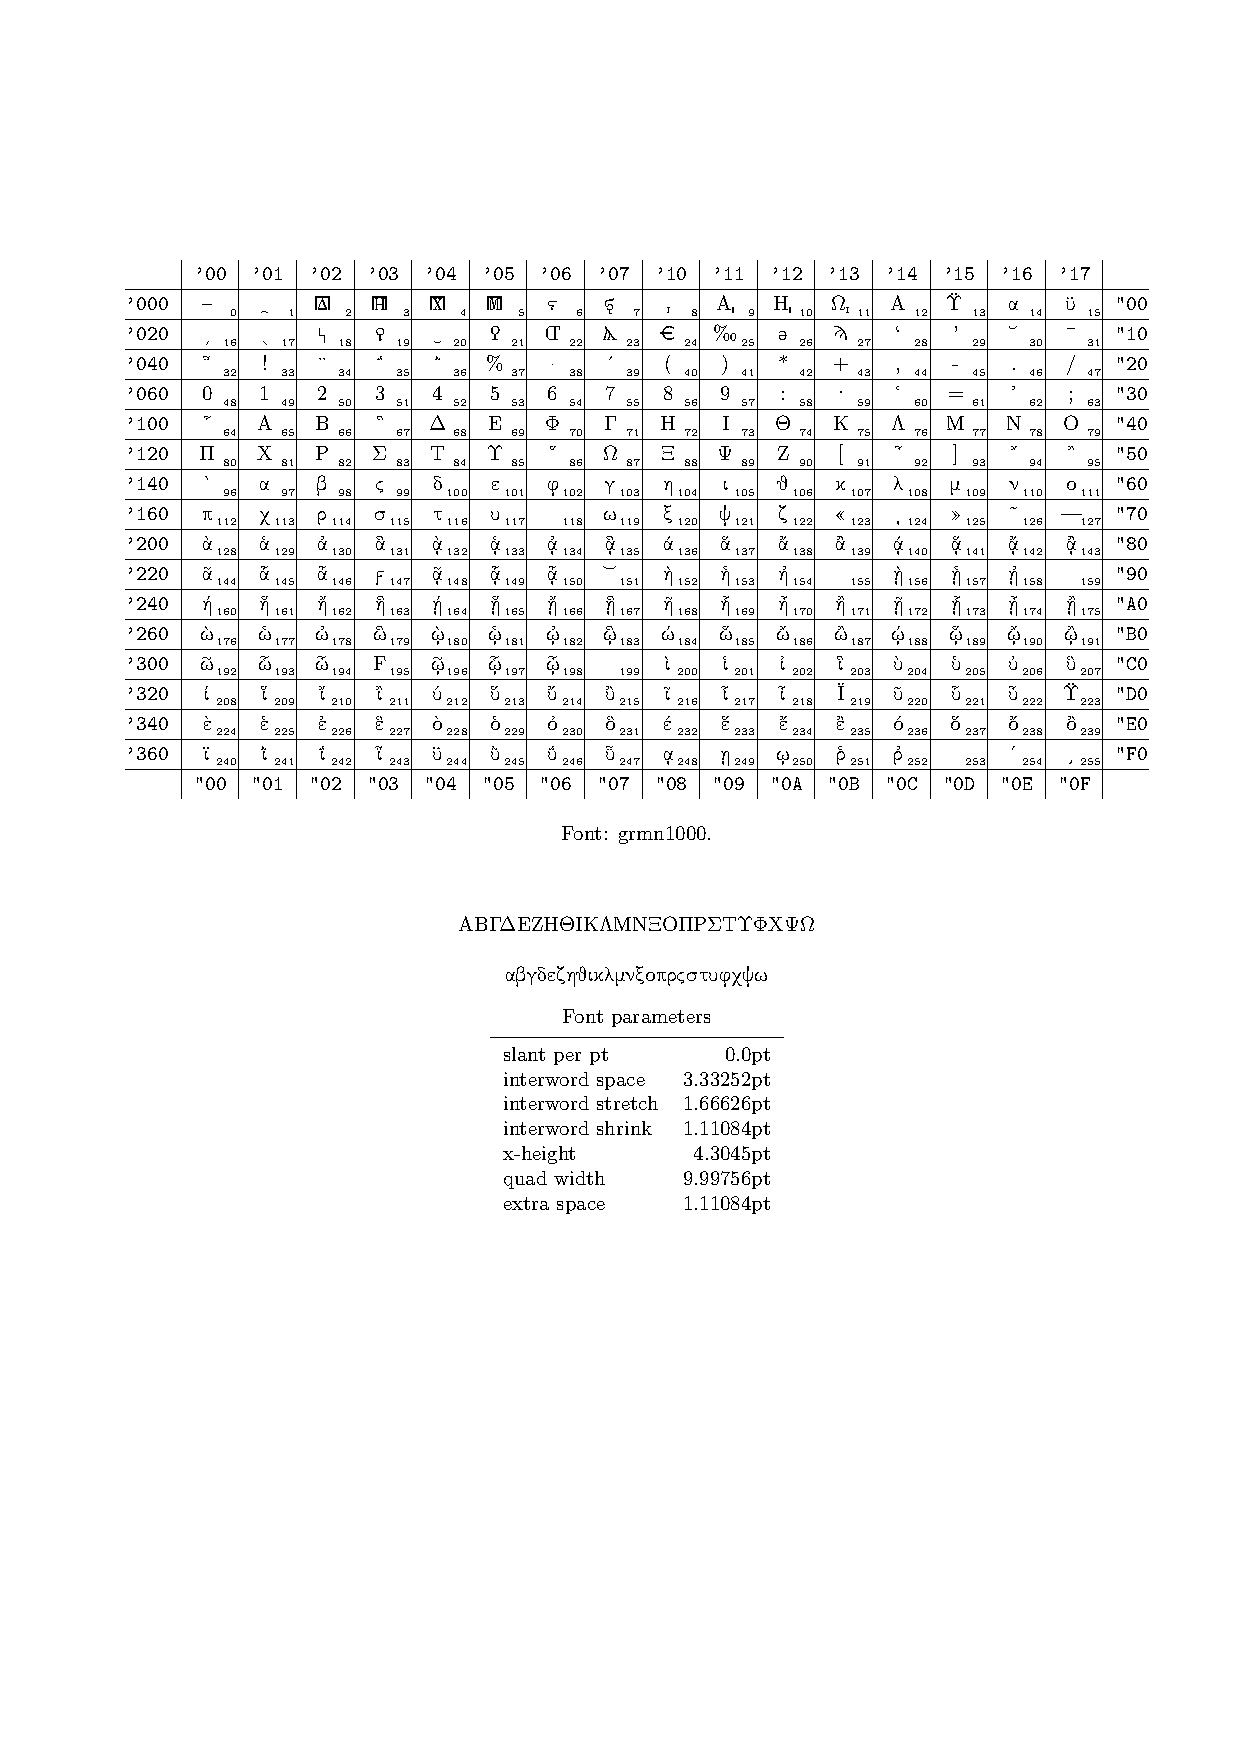
\includegraphics{grmn1000table}}
\caption{The layout of the textual CB Greek fonts}\label{fig:grmn}
\end{figure}

\section{Known bugs and features}
I admit that when I wrote the macros that make the CB Greek fonts usable I believed that I could get along without caring of other packages. This was an evident mistake, and while I keep maintaining the fonts and the \textsf{teubner} package, I try to overcome the incompatibilities that are gradually showing up.

Certainly the clash between the \verb|\digamma| command of \textsf{amsmath} and friends with the homonymous command of the Greek language, did show itself from the very beginning, when Apostolos did prepared the \textsf{babel} language description file for the Greek language; since the early tests, it was evident it was necessary to define different commands. In facts for using the lower and upper case digamma signs in Greek, \foreignlanguage{greek}{\ddigamma, \Digamma}, it is necessary to use respectively the commands \verb|\ddigamma|, and \verb|\Digamma|, none of which clashes with \textsf{amsmath} and friends. The \textsf{teubner} package adds \verb|\f| and \verb|\F|.

Unfortunately the \textsf{teubner} package introduces several other clashes with the commands defined in \textsf{amsmath} and friends;  work is in progress in order to spot them and find suitable corrections. 

Users are therefore kindly requested to inform me about such clashes and/or clashes with other packages; if possible they should accompany their bug notification with a minimal example and/or, if they discovered the cause, the description of the cause of the clash. Please refer to my home e-mail address:
\begin{quote}\ttfamily
claudio dot beccari at alice dot it
\end{quote}

\section{The fonts}
Table~\ref{fig:grmn} shows the layout of the normal text Greek font inspired by the Didot design; most of the glyphs were designed by Silvio Levy, but all of them were revised; in particular the ligature mechanism with the two species of sigmas were completely redone, so as to have many more slots for accented characters.

Table~\ref{tab:famsersha} displays the families series and shapes available with the CB Greek fonts. It's worth noting that all families have some series and/or shapes that are absent into the regular EC fonts. On the opposite there are some series and/or shapes missing from the LM fonts; the latter contain for example the slanted version of the caps and small caps, but, at the moment they do not contain the bold caps and small caps. The LM fonts contain also some demi bold condensed versions that here are available only for the Lipsian shape. 

The user should not worry too much about these inconsistencies, in the sense that if s/he asks for a missing shape or series, the typesetting engine will inform him/her in the log file of what is missing and what it has been substituted. In spite of these deficiencies, the user may keep in mind that the EC, LM and CB collections contain more families, series and shapes that most commercial fonts. For what concerns the CB fonts, it is not unlikely that new series and shapes will be designed in the future; for the moment it is necessary to do with what is available now, which is satisfactory for most typesetting works.


\begin{table}[htb]
\def\R#1{\rotatebox{90}{#1}}
\def\V{\rule{0pt}{2.5ex}}
\centering
\begin{tabular}{rccccccc}
						& \R{regular}	& \R{outline}	& \R{sanserif}	& \R{typewriter}	& \R{slides proportional} 	& \R{slides monospaced}	& \R{metrae}	\\\hline
upright shape\V			& m, bx			& m, bx			& m, bx			& m				&							&						& m			\\
slanted shape			& m, bx			& m, bx			& m, bx			& m				&							&						&			\\
upright serifed shape	& m, bx			& 				&				&				&							& 						&			\\
slanted serifed shape	& m, bx			& 				&				& 				&							&						&			\\
italics shape			& m, bx			& m, bx  		& m, bx			& m				&							&						&			\\
Lipsian italic shape		& m, b, bx		& 				&				&				&							&						&			\\
upright italics shape	& m, bx			&  m, bx 		& m, bx			& m				&							&						&			\\
italics variant			&				&				& m, bx			&				&							&						&			\\
upright italics variant	&				&				& m, bx			&				&							&						&			\\
small caps shape			& m, bx			& m, bx  		& m, bx			& m				&							&						&			\\
visible 					&				&				&				&				& m, bx						& m						&			\\
invisible				&				&				&				&				& m, bx						& m						&			\\
visible					&				&				&				&				&							& 						&			\\
invisible				&				&				&				&				&							& 						&			\\\hline
\end{tabular}

\caption[Families, series and shapes available with the CB Greek fonts]{Families, series and shapes available with the CB Greek fonts. Each table slot contains the  symbols for `medium', `bold', and `bold extended' when they are available for that particular family and shape that label the respective rows and columns.}\label{tab:famsersha}
\end{table}

\section{Legalese}
This work may be distributed and/or modified under the conditions of
the \LaTeX\ Project Public License, either version 1.3 of this license or
(at your option) any later version. The latest version of this license
is in \begin{quote}
\texttt{http://www.latex-project.org/lppl.txt} \end{quote}
and version 1.3 or later is
part of all distributions of \LaTeX\ version 2003/12/01 or later.

This work is made up of the map file \texttt{cbgreek-full.map}; of 1034 \MF\ source files individually labelled as belonging to the CB Greek font collection; of 944 \TeX\ metric files derived from the \MF\ sources; of 944 type~1 font files in pfb format; of this file \texttt{cbgreek.pdf} you are presently reading, together with its source file \texttt{cbgreek.tex} and the included graphics file \texttt{grmn1000table.pdf}; of the font description files that match those of the T1 encoded LM fonts.

The encoding file CB.enc was prepared by Apostolos Syropoulos for his rendering in pfb format of my \MF\ fonts at the only size of 10\,pt. I modified a little the file comments related to some particular CB glyphs or certain specific positions of the CB fonts, but the substance is by Apostolos. The font description files whose names start with \texttt{lgrcm} or \texttt{lgrlcm} are distributed with \textsf{babel} and were originally prepared by Apostolos Syropoulos, before Johannes Braams verified them and included them into his bundle. I modified the \texttt{lgrcmr.fd} and \texttt{lgrcmss.fd} font description files in order to accommodate the new shapes\footnote{By the way, the original \texttt{fd} files contain a warning that modifications can be made bat the modified files cannot be distributed with the same name. This warning applies to all files distributed with the \textsf{babel} bundle, but this restriction cannot be applied to the \texttt{fd} files, because their name \emph{has to be} built up with the agglutination of the encoding and the family names.}.

The copyright of the source \MF\ files is mine, but without the support of Apostolos Syropoulos I would have done nothing; much of what I put in the source files derives from Apostolos; I therefore hereby declare that he shares with me all the rights of the copyright holder.

\section{Acknowledgments}
I  have to thank many people and I can't list all of them here, but some
are so important that I have to specify:

Silvio Levy produced the first Greek font files I started with; if I had
to start from scratch my fonts wouldn't even exist.

Yannis Haralambous wrote other \MF\ files after those of Levy; I got
suggestions also from Yannis files. He gave me also very fine advice and
suggestions, for which I thank him in a special way.

Jorge Knappen produced the EC fonts  from  which I got the whole idea of
extending that approach to the Greek fonts; for  compatibility  reasons,
therefore,  I  extracted  his  METAFONT  interpolation routines from his
files and put them  in  the  file  cbspline.mf;  the merit of generating
fonts of any size between 5pt and 99.99pt comes directly from Jorge.

Apostolos Syropoulos, the president of the Hellenic Association  of  the
Friends  of  \TeX,  assisted me with patience and countless suggestions,
criticism and time spent in  testing  the various versions of the fonts.
He also was the first one who dared using my fonts, and, he told me,  he
started with the slides for  a  speech  he  gave some years ago, when no
other Greek slide fonts were available.  He also wrote the  experimental
versions  of the \textsf{babel} extensions for the Greek language and defined the
font definition files that go with version 3.7 of \textsf{babel}.

Dimitri Filippou tested my  fonts  and  sent  me a conspicuous number of
suggestions and criticism  for  which  I  thank  him  very much. He also
"forced" me to produce the Lipsian Greek fonts; he  cooperated  in  this
task revising the different glyphs several times; he spent a lot of time
helping  me  with  these  fonts;  without his help the Lipsian fonts would not
exist. Later on he helped me with  the revision of  the sans serif fonts
and revised every single lower case glyph in this family. Again a lot of
thanks.

The many unknown Hellenic Friends of \TeX\ who, with the intermediation of
Apostolos,  let me know the bugs of the \MF\ code I wrote, so that I
could correct it and possibly eliminate some of those bugs.

\enlargethispage*{3\baselineskip}
\section{Maintainance}
I intend to maintain the work, although, when I redid this transformation, 
I discovered so many imperfections in the smaller optical sizes, that possibly I 
have to start from scratch.

\bigskip

\noindent 
4 January 2008\hfill Claudio Beccari

\end{document}

\noindent\cbtest[\uishape]\\
\cbtest[\lishape] \cbtest[\fontseries{b}\lishape] \cbtest[\fontseries{bx}\lishape] \\
\cbtest[\rsshape]\\
\cbtest[\roshape]\\
\sffamily
\cbtest[\uishape]\\
\cbtest[\ivshape]\\
\cbtest[\uvshape]







